\documentclass[a4paper,10pt, twocolumn]{article}
\usepackage{amsmath}
\usepackage{graphicx}
\usepackage[font={small,it}]{caption}

\begin{document}

\title{Neural Networks for Time Series Prediction}
\author{Alun Meredith}
\maketitle

\begin{abstract}

\end{abstract}
\section{Neural Networks}
Neural networks follow a model inspired by the mechanisms of neurons and dendrites in biological brains. Composed of an array of 'nodes' which map a signal with a simple activation function into a single output.

In feed forward networks the nodes are connected hierarchically and the signal feeds through each layer of nodes; each contributing their signal forward weighted to each node in the next layer. By constructing these weighted sums of many different combinations of the input variables even a single layer neural network can model complex dependencies.  

Training a neural network is a matter of finding the appropriate map of weights connecting each node together. However the error function here is often high variance with local minima which makes it more difficult to train. To get around this activation functions with mathematical properties are often used to make sure the error function is convex and a backward propagation algorithm iterates the error. 

The backward propagation algorithm works very similarly to the feed forward in that we don't know the error from the first layer of a neural network but we can calculate the error from the last layer and subtract it from the total error and propagate the remainder backwards. 

\subsection{Two Class Classification}
We describe a familiar problem, classifying two multivariate normal distributions with unequal covariances as shown in figure (\ref{fig:NNcontours}a). The means and covariances used are given below:
\begin{align}
	\mathbf{m_1} = [0 \;\; 3]^t \qquad \mathbf{m_2} = [4 \;\; 0]^t \\
	\mathbf{C_1} = 
	\begin{pmatrix}
	2 & 1 \\
	1 & 2
	\end{pmatrix} \quad
	\mathbf{C_2} = 
	\begin{pmatrix}
	1 & 0 \\
	0 & 1
	\end{pmatrix}	
\end{align}

\begin{figure}[ht]
	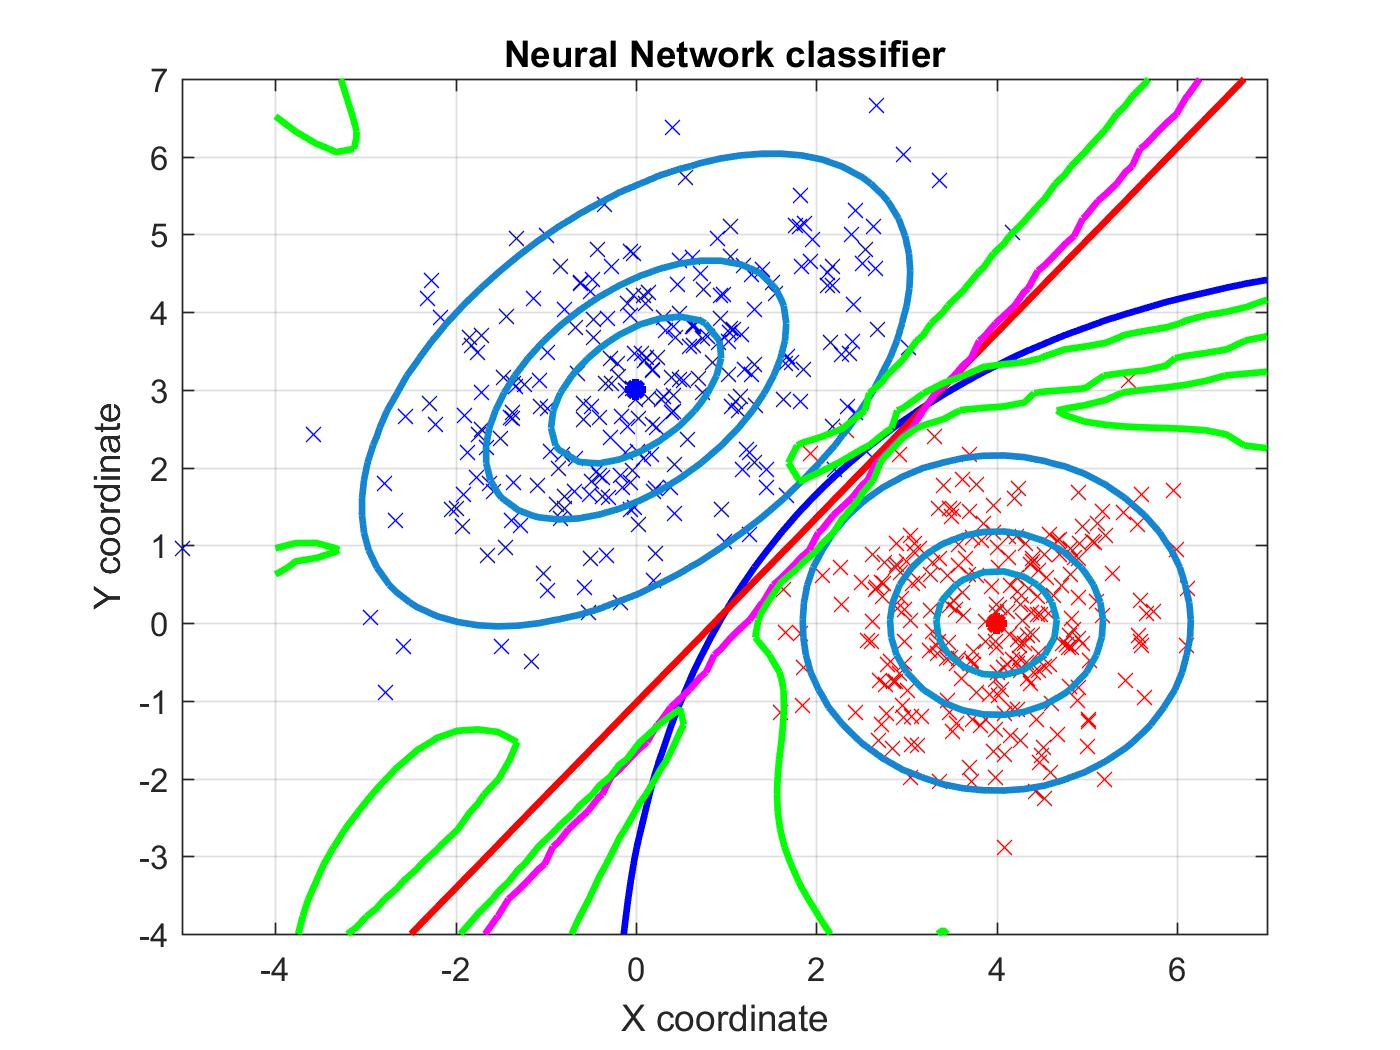
\includegraphics[width=0.9\linewidth]{NeuralNetworkClassification.jpg}
	\centering
	\caption{$p=0.5$ classification boundaries of two multivariate Gaussian distributions sampled 200 times. Blue - Posterior probability. Magenta, Red, Green are single layer feed forward networks using Bayesian regularisation with 3,20  and 80 nodes respectively }
		\label{fig:NNcontours}
\end{figure}

\begin{figure}[ht]
	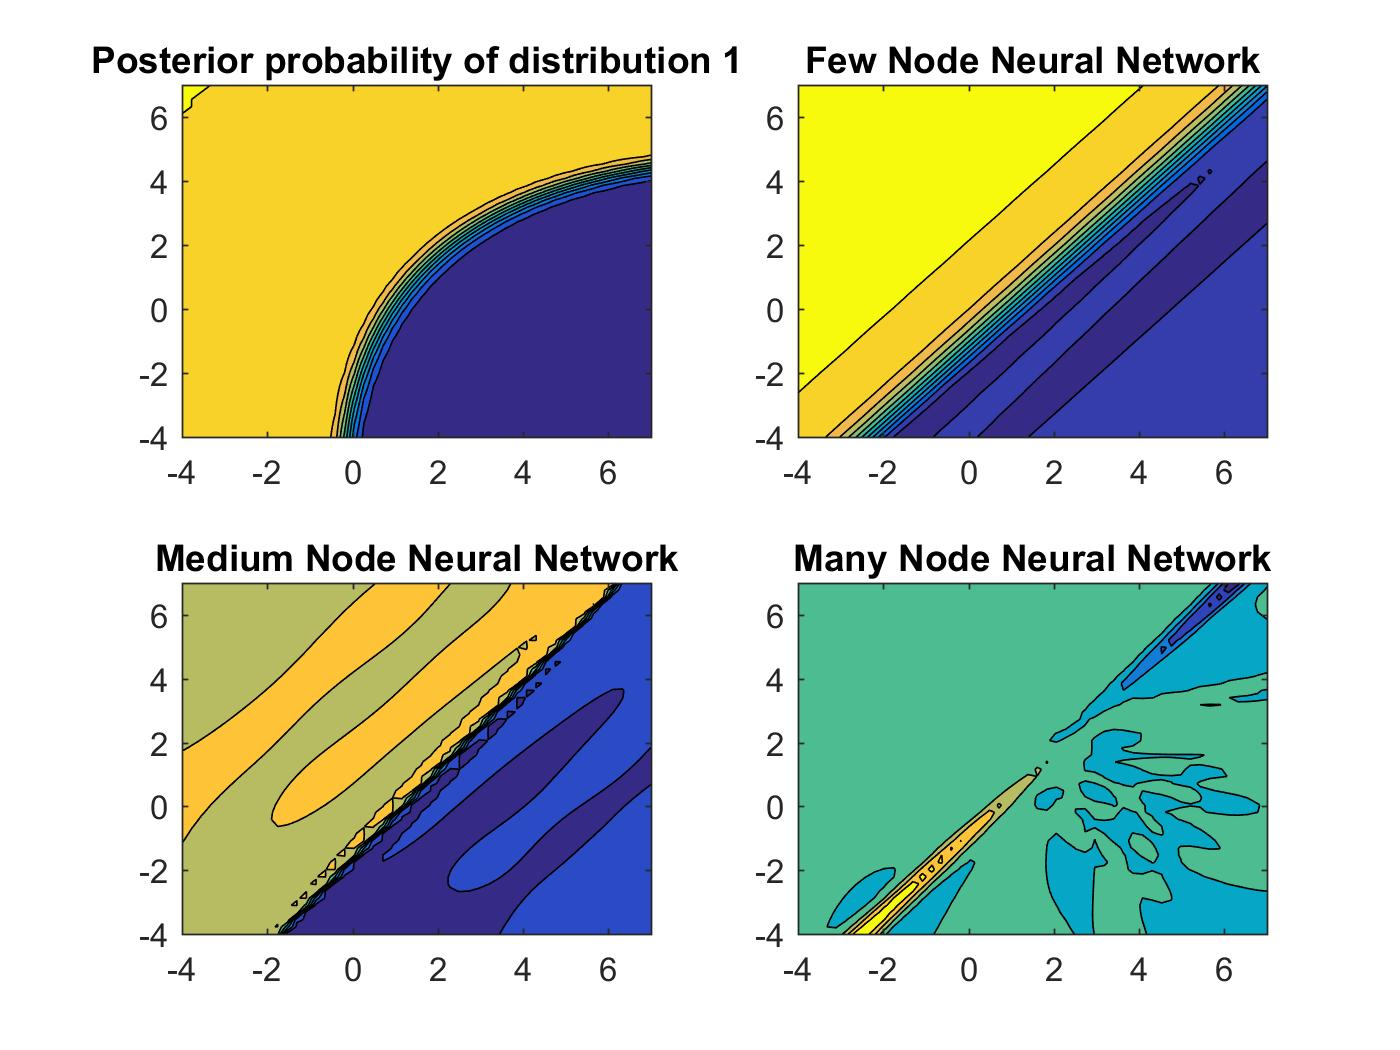
\includegraphics[width=0.9\linewidth]{neuralNetSurf.jpg}
	\centering
	\caption{Top Left: Posterior probability for distribution 1 and prediction for 3,20 and 80 node single layer feed forward neural network using Bayesian regularisation for top right, bottom left and bottom right respectively }
		\label{fig:NNsurf}
\end{figure}

\begin{figure}[ht]
	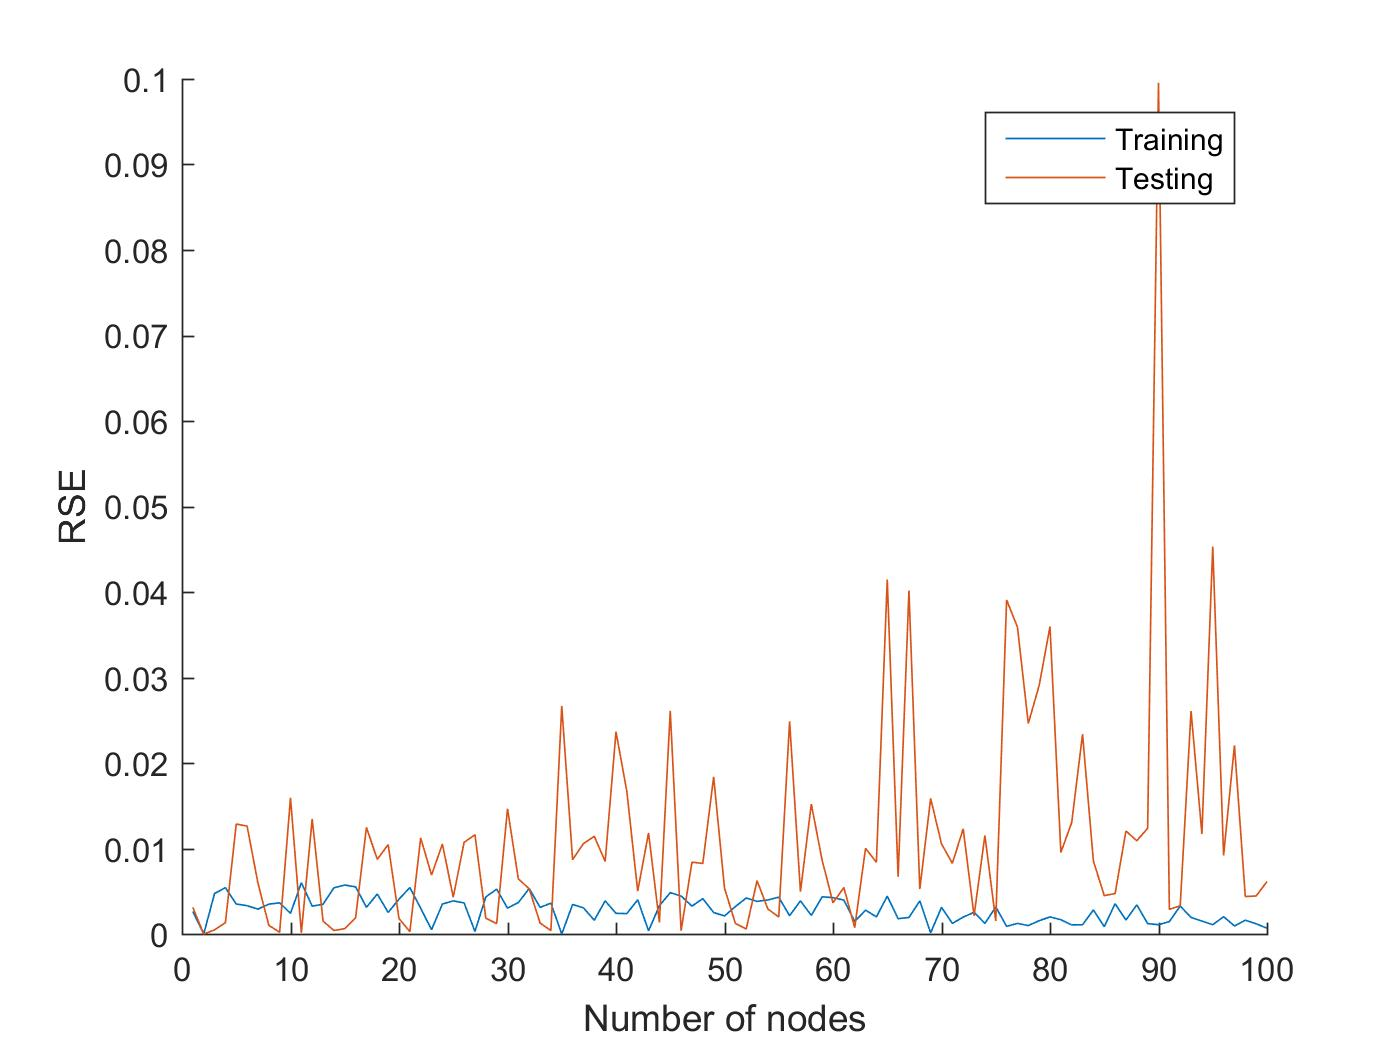
\includegraphics[width=0.9\linewidth]{nnErrorVar.jpg}
	\centering
	\caption{Relationship between training set and testing set error for a single layer feed forward neural network classifying the distributions described in eq.(1,2) with Levenverg-Marquardt gradient descent }
		\label{fig:NNnodes}
\end{figure}

\begin{figure}[ht]
	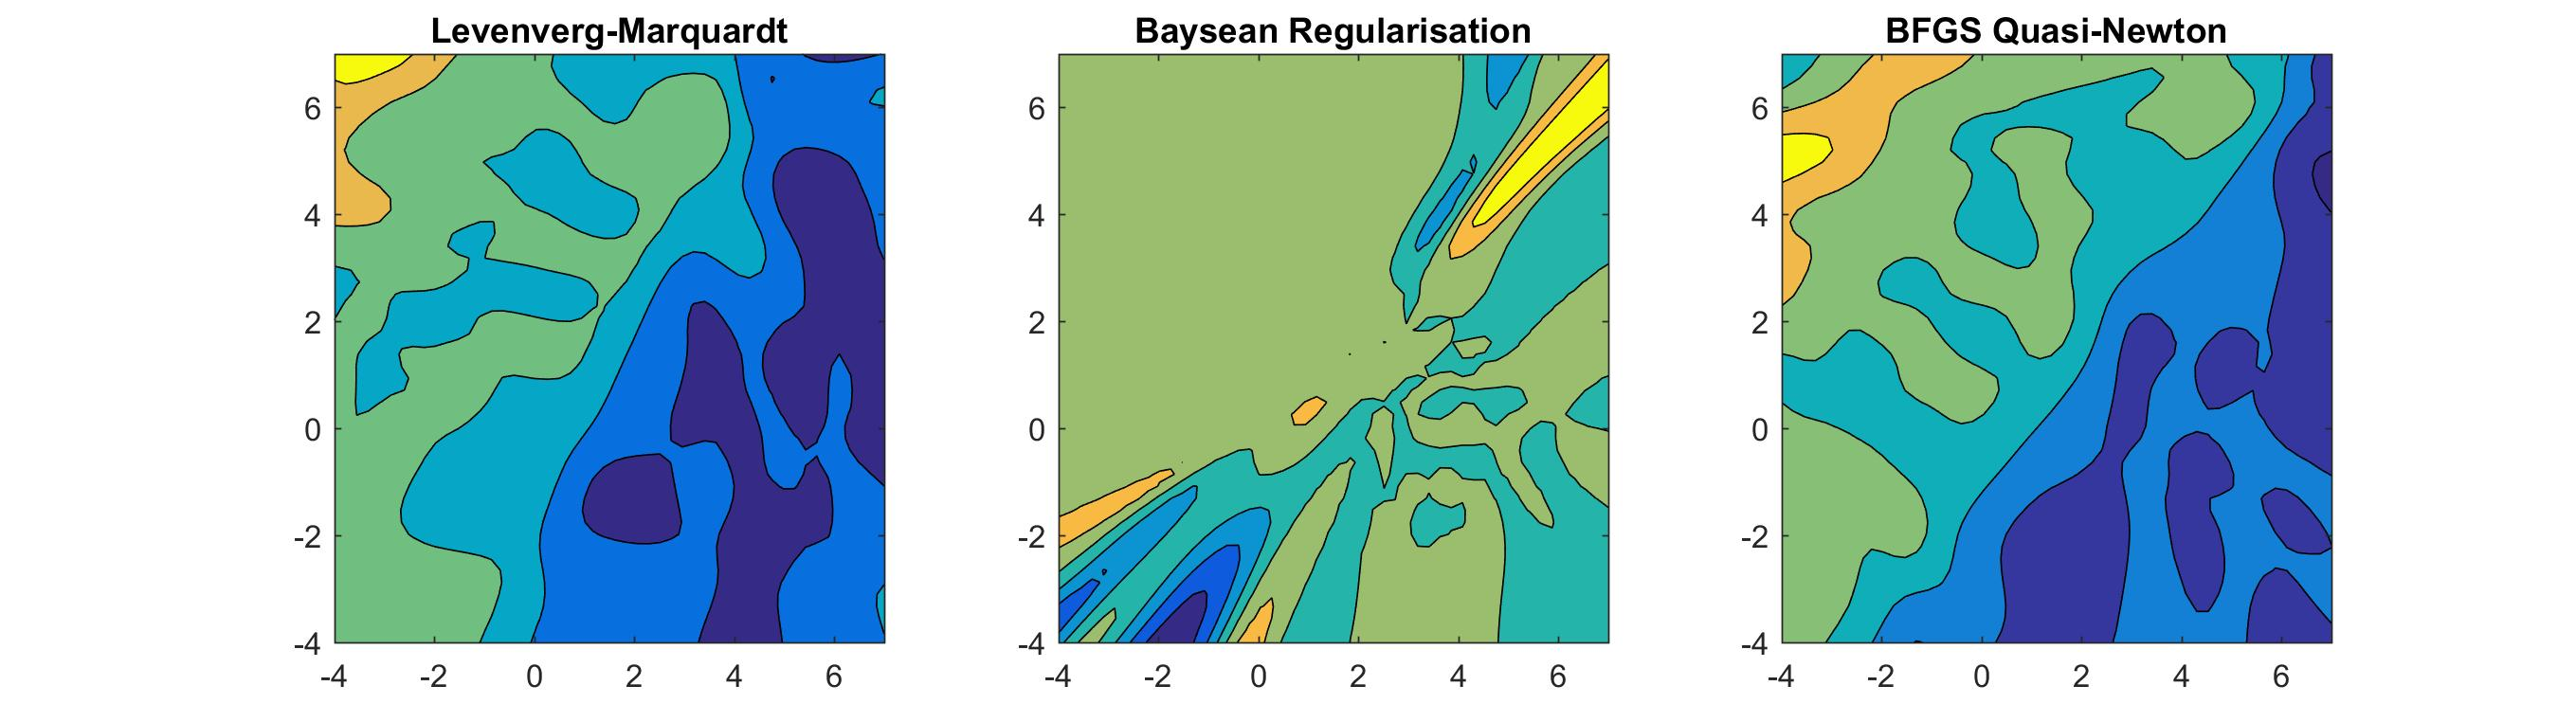
\includegraphics[width=0.9\linewidth]{nnAlg.jpg}
	\centering
	\caption{Prediction heat maps of 3 different training algorithms: Levenverg-Marquardt(left), Bayesian Regularisation(centre) and BFGS Quasi-Newton gradient descent}
		\label{fig:NNalg}
\end{figure}

The ability for a neural network to produce complex functions is a product of the size of structure of the nodes within it. A single node is only capable of producing a single activation function (sigmoid) function (high bias) but a single neural layer with the same number of nodes as training data is capable of having a single node represent each training data point. Needless to say this like all other learning methods when the model complexity increases produces high variance results.

This relationship between network size and variance/bias shown in (fig.\ref{fig:NNsurf} and fig.\ref{fig:NNcontours}), where we see a bias for linear discrimination in the small structure networks but variance in the larger neural network. Figure(\ref{fig:NNnodes}) shows the relationsip between number of nodes in a single layer network with variance through changes in training in testing set error. Although noisy due to low numbers of data the training error continues to decrease over time while the testing error generally increases from somewhere in the range of 10-30 nodes. 

In order to combat high variance there are many familiar and non - familiar techniques. Cross validation, reducing the size of the neural network and regularisation and adding noise to the input ("jitter"). 

Different algorithms for gradient descent also produce different results, figure (\ref{fig:NNalg}) shows heatmaps for 4 different training functions. These differ partially because some algorithms get caught in local minima and others use some of the variance combating techniques measured above such as the Bayesian regularisation algorithm. 

\section{Chaotic Time Series}

As discussed overfitting can be a large problem for neural networks when trying to generalise on noisy data due to the complex network being able to produce complex models. However in some domains this can be a benefit. Here we consider the ability for a neural network to predict a chaotic time series and compare it to a linear regression model. 

Chaotic systems are highly sensitive to the initial conditions but fundamentally deterministic. Which makes it both difficult to generalise but also also possible although hard to predict to extreme accuracy. The Mackey-Glass model is a good example of this and capable of giving sustained oscillatory signals (figure \ref{fig:Mackey-Glass}). It is the solution to the differential in eq.3. 

In a time series we have taken the last 20 data points to produce the features of a linear model(\ref{fig:Mackey-Glass}) and compared this to the result of a neural network (\ref{fig:nnMackeyGlass}.) In  figure \ref{fig:Mackey-Glass} the real time series (test set) is obscured by the one step prediction line. This line predicts a single data point and then recalculates its weights based on the change. Unlike the feed forward algorithm. In the feed forward algorithm predicted datapoints are fed into the system to be used as the initial condition for the point after that and so on. This causes the accumulation of errors which for a chaotic system highly dependent on its starting conditions means that very quick divergence. 

An interesting feature of the time series prediction is the duration in which the algorithm "remembers" i.e. the number of previous data points in which the prediction value is evaluated. Figure \ref{fig:linMemory} shows how the RMSE changes as the feature set is expanded to these earlier points. Intuition tells us that more complex features lead to the ability to produce more complex functions and overfitting. We can see from the graph that there is a breakpoint at 170 iterations (17 units of time) which is equal to the value of $\tau$ used. 

Finally we repeat the process of training one step predicting and free running prediction for a Neural network of twenty nodes.(fig.\ref{fig:nnMackeyGlass}) While the one step prediction remains very accurate the free running mode looks quite different from the test data. It has produced high frequency sustained oscillations demonstrating these are possible. However it is hard to justify this as more accurate than the linear model which maintained a structure that looked more familiar to the function. Of course accuracy is not a particularly interesting statistic to judge these the performance of the free running models due to the highly chaotic and diverging nature, however we can compare the training set and testing set accuracies of the models. 

Table 1 shows that the linear regression performs much better on the training set while one step error is roughly equivalent. It seems that the neural network struggles to accurately model the periodicity of the function as it is able to make short term accurate predictions but fails to even fit the training data to an equivalent order to the linear regression. I would hypothesise that this is due to the structure of the features in the two models. The linear models can easily capture high order linear terms and produce smooth curve but the neural network must approximate these curves by summing together a set of sigmoid functions. Altough it is possible to capture these functions completely with an adequately sized single layer neural network good approximations would take a large array of nodes. 
\begin{align}
	\frac{dx}{dt}= \frac{ax(t-\tau)}{1+x(t-\tau)^{10}}-bx(t)
\end{align} 	
	
\begin{figure}[ht]
	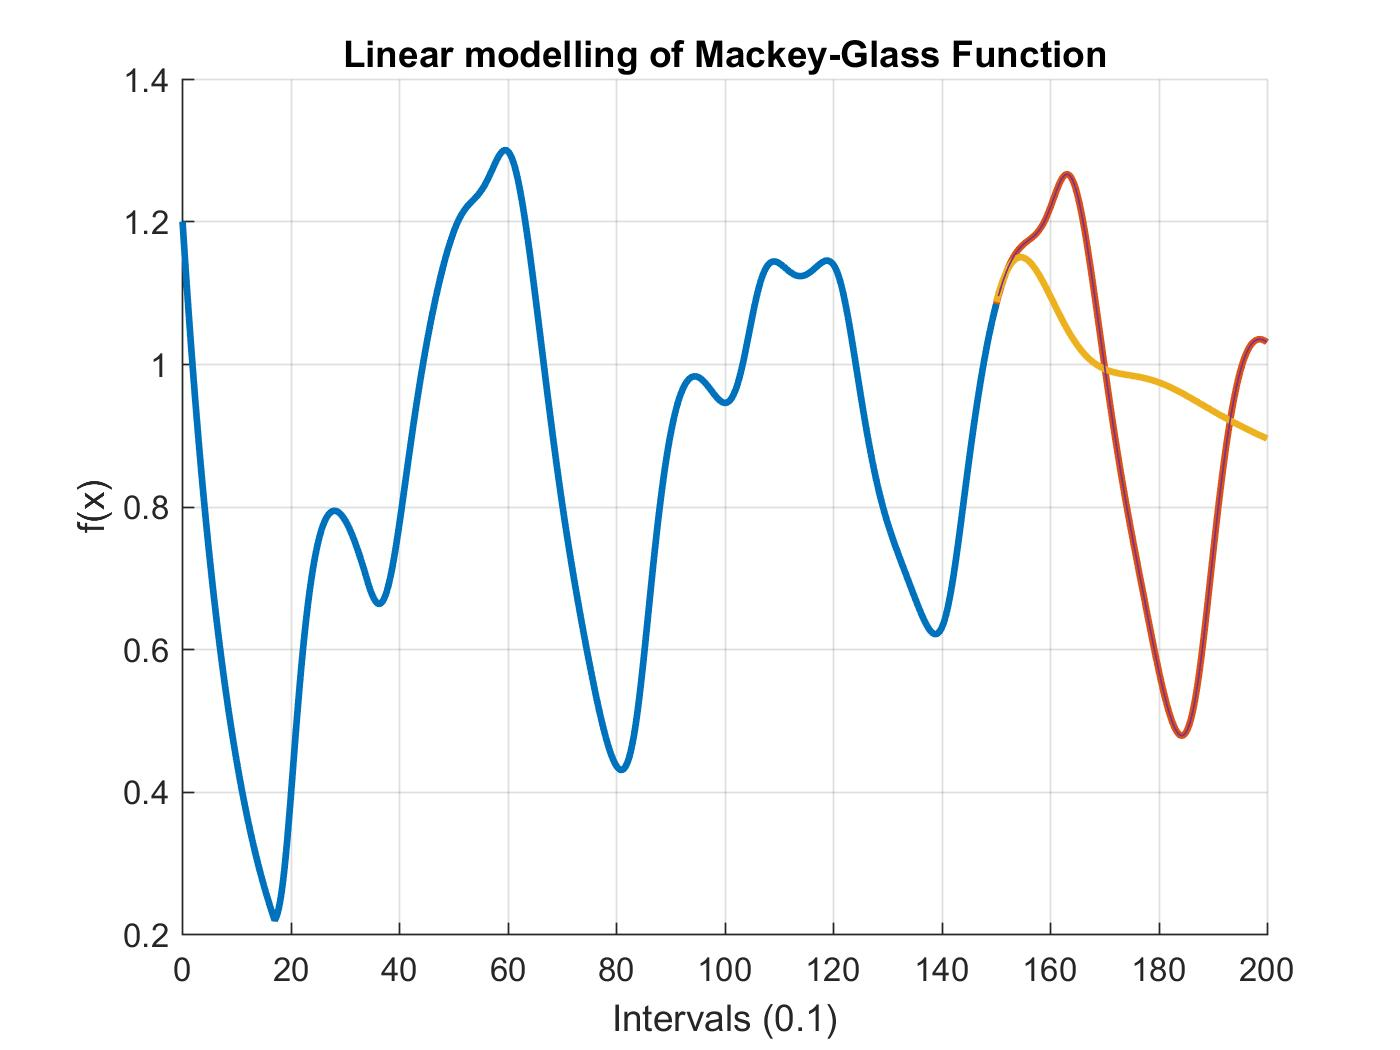
\includegraphics[width=0.9\linewidth]{mackeyGlass.jpg}
	\centering
	\caption{Mackey-Glass time series over an interval of 200, First 150 observations given as training data (blue line), One step prediction (red) and free running prediction (yellow)}
		\label{fig:Mackey-Glass}
\end{figure}

\begin{figure}[ht]
	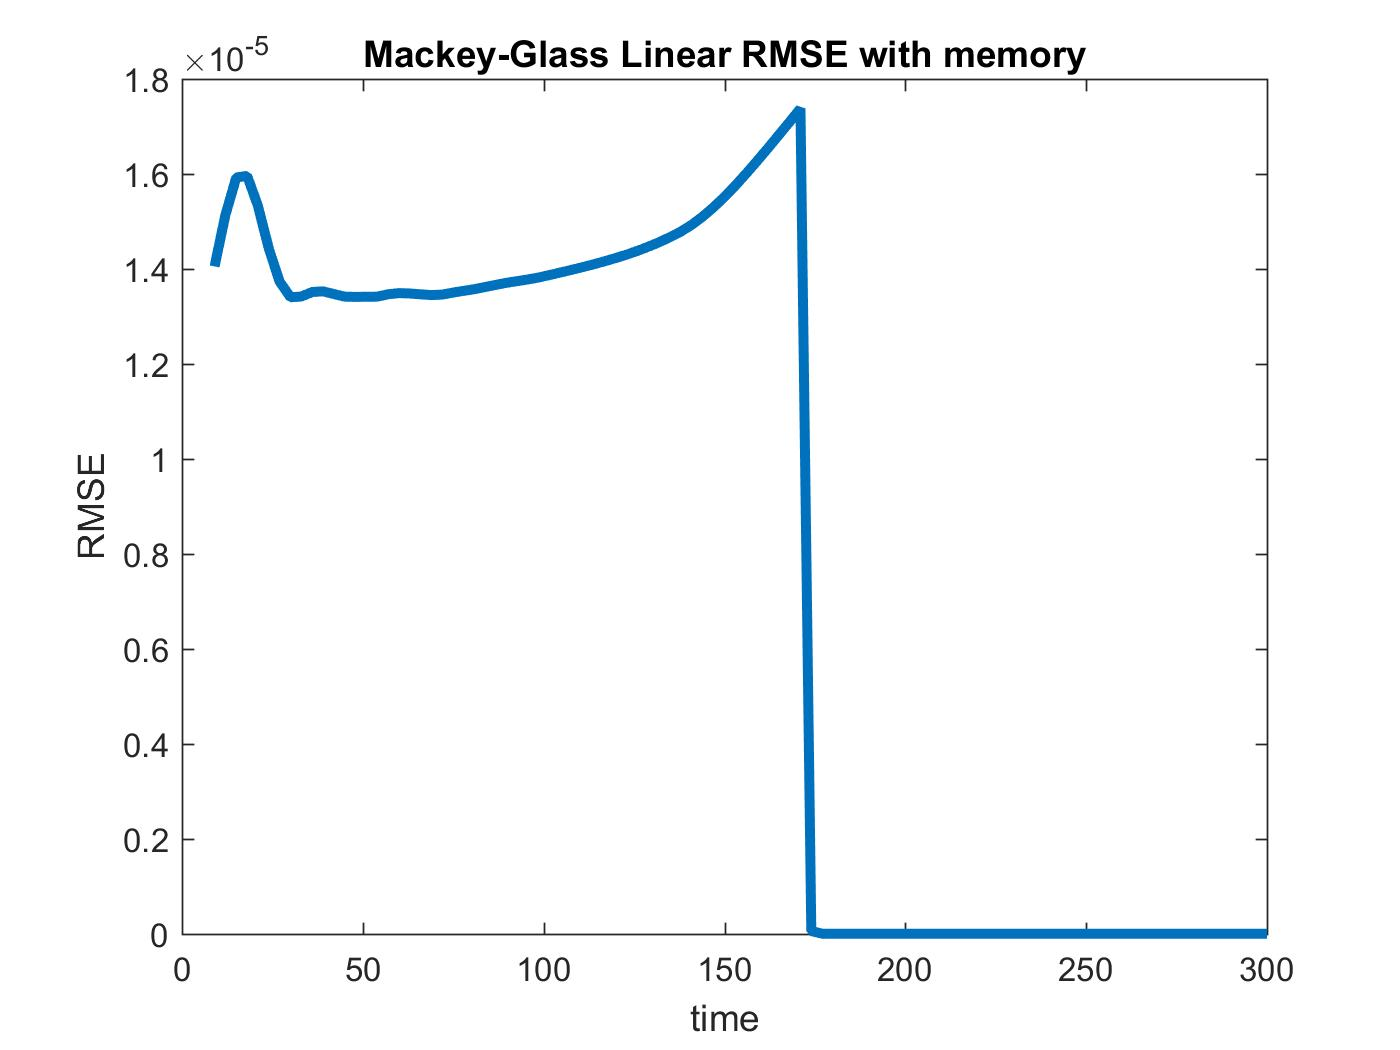
\includegraphics[width=0.9\linewidth]{linMemory.jpg}
	\centering
	\caption{ Change in root mean square error for an 80 node single layer feed forward neural network to characterise the Mackey Glass equation for a $\tau$ of 17 as a function of time "remembered".  }
		\label{fig:linMemory}
\end{figure}
\begin{figure}[ht]

	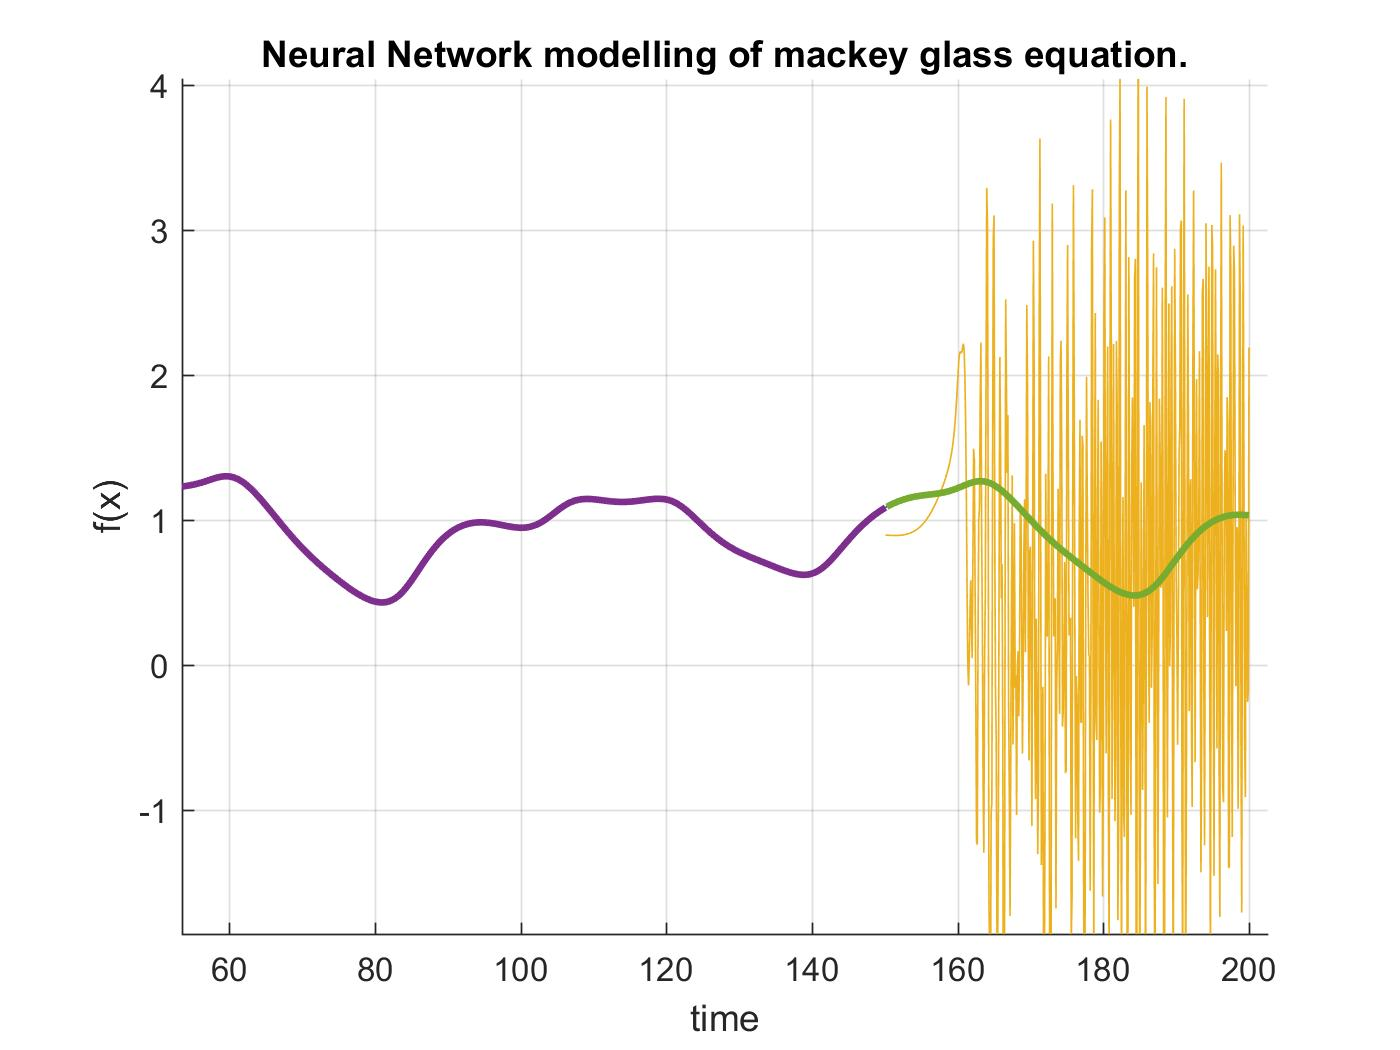
\includegraphics[width=0.9\linewidth]{nnMackeyGlass.jpg}
	\centering
	\caption{ Prediction values of a 80 node neural network t modelling Mackey-Glass with a $\tau$ of 17 for both training set (purple), one step prediction(green) and free flowing linear algorithms (yellow)  }
		\label{fig:nnMackeyGlass}
\end{figure}

The average RMSE of data in the one step prediction is $1.5942e-05$. 

\begin{table}[b]
\begin{tabular}{l c|c|c|c}
	
	& Train & One Step & Free  \\
Linear Regression & 1.56e-05 & 3.56e-04 & 0.182 \\
Neural Network &  2.50e-03 & 3.83e-04 &  1.10 \\
\end{tabular}
\caption{RMSE for 80 node 1 layer feed forward neural network and linear regression predicting the Mackey-Glass time series ($tau =17$); predicting on the training set, iterative one step prediction and Free running prediction }
\end{table}

\section{Financial Time Series}
As seen in the last section, neural networks can struggle to capture chaotic systems in a free running mode as errors accumulate quickly causing divergence. However our neural network was accurate for the one step predictions. We will attempt to replicate that in the non-deterministic space of the stock market. 
\begin{figure}[ht]
	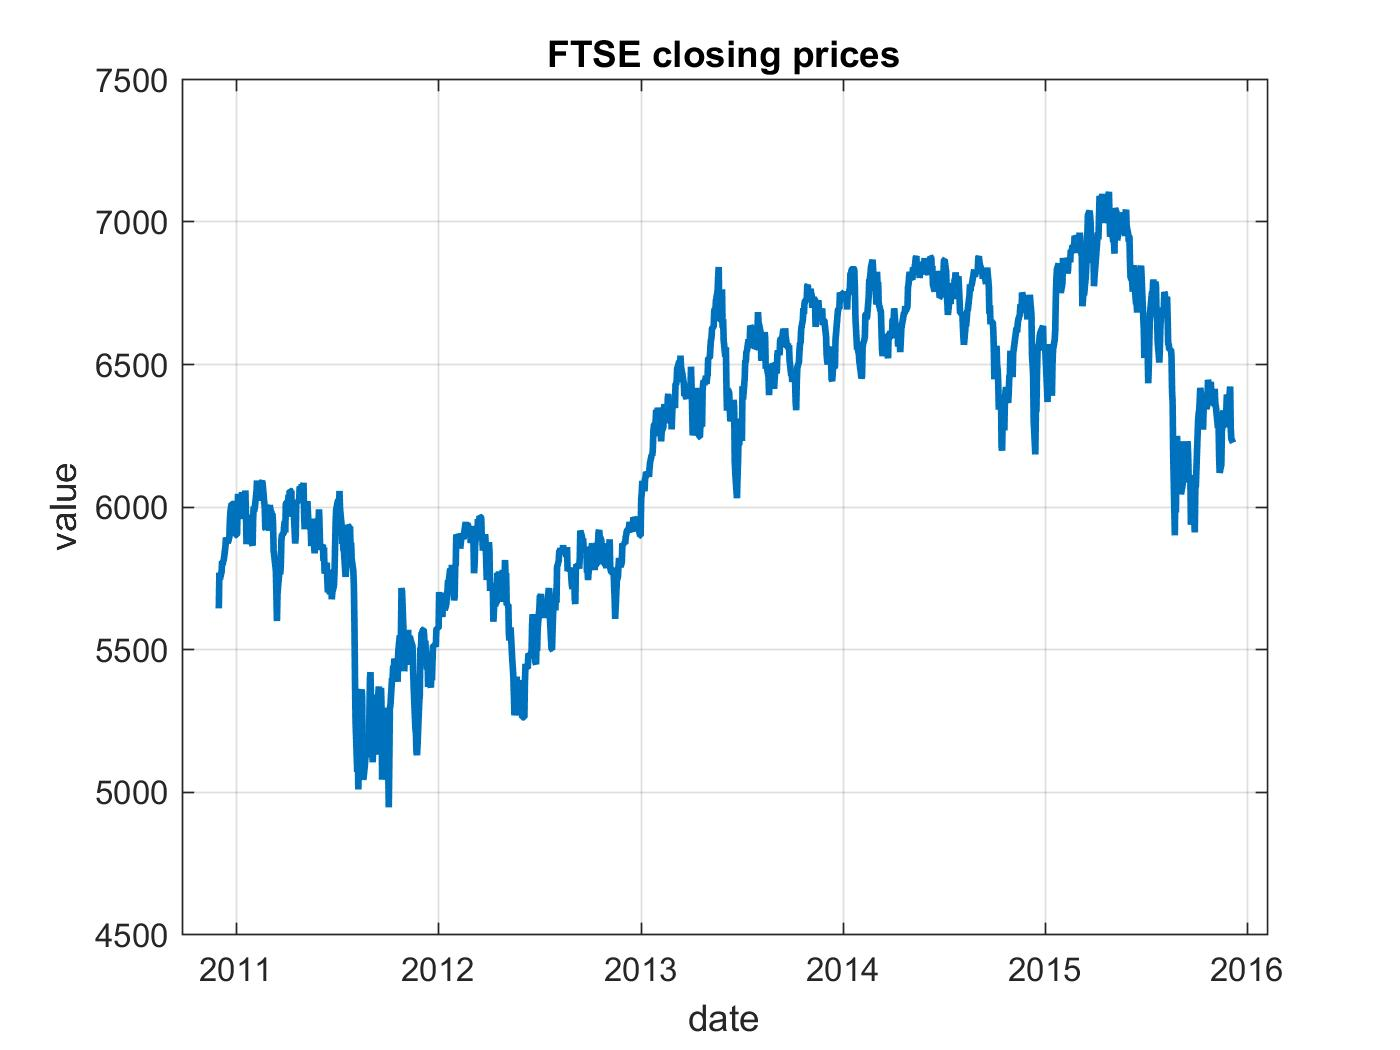
\includegraphics[width=0.9\linewidth]{FTSEclose.jpg}
	\centering
	\caption{ FTSE closing prices for the last year  }
		\label{fig:FTSEclose}
\end{figure}

\begin{figure}[ht]
	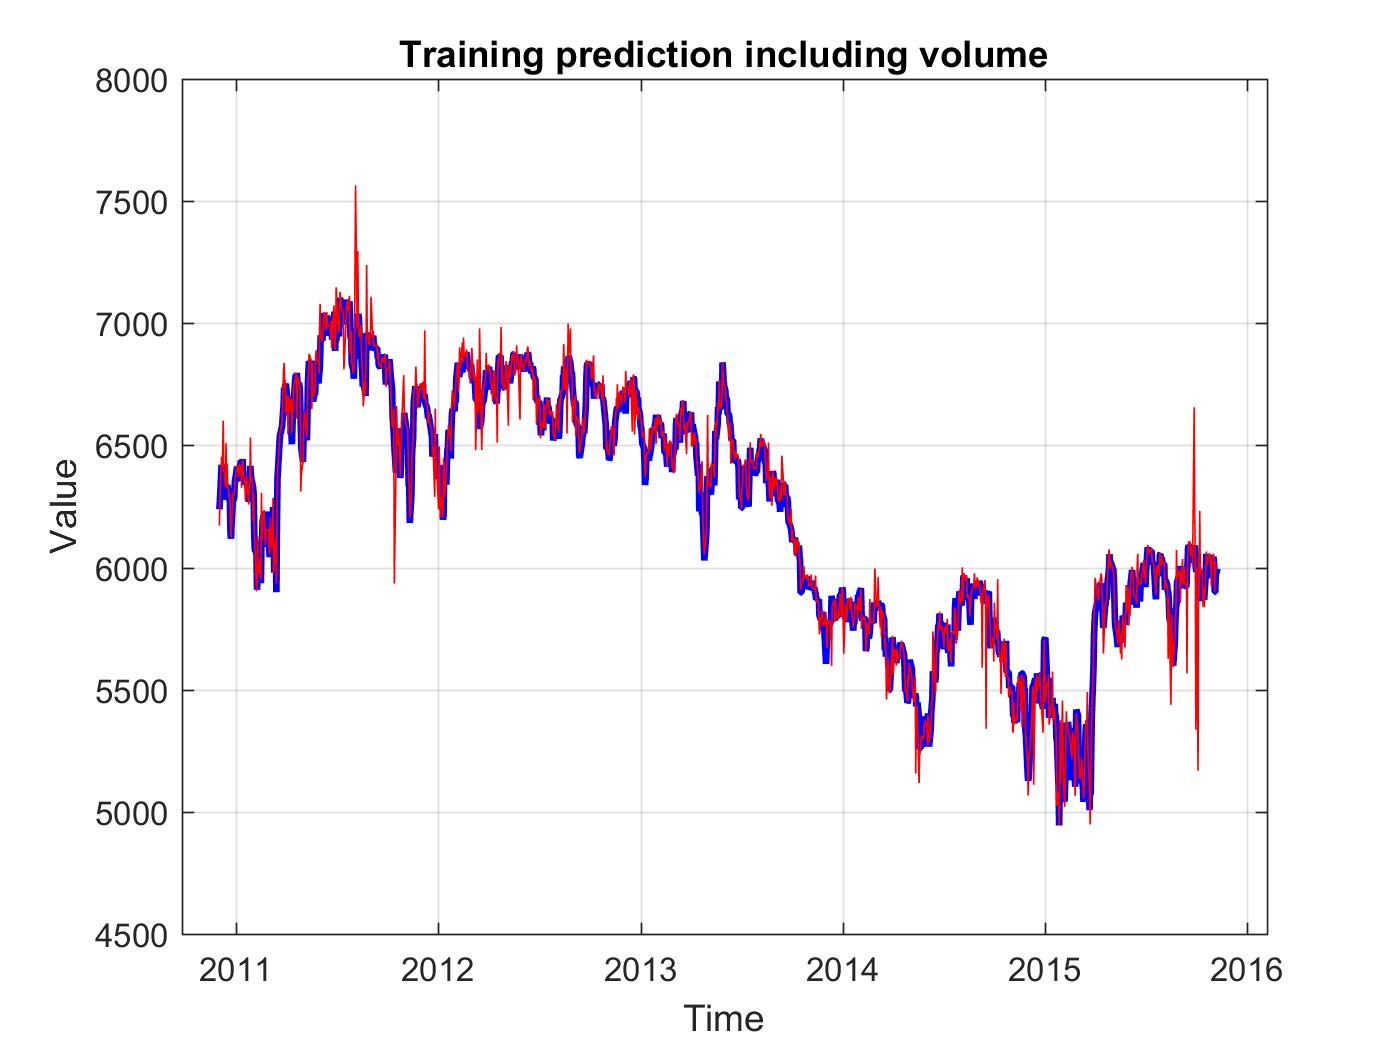
\includegraphics[width=0.9\linewidth]{FTSEtrainVol.jpg}
	\centering
	\caption{ FTSE internal training prediction of [30 30 30] nodes 3 layer network using Bayesian regularisation. Including volume of trades information }
		\label{fig:FTSEtrainVol}
\end{figure}
In the first part to this lab strong generalisation was an important feature to the model as the sampling was largely random noise, in the second part very high over-fitting was sought after as complex but deterministic patterns require equally complex models to capture. This last application requires a balance of the two as financial markets are both highly complex but also noisy. The closing value of the FTSE for the last 5 years and last 40 days are shown in figure \ref{fig:FTSEclose} and \ref{fig:FTSEclose40} respectively. 

We will only consider the one step prediction model and considering the difficulty proposed by predicting a stock market we can try to achieve a balance of bias and variance through a complex node structure incorporating regularisation. 

Figures \ref{fig:FTSEclose} show the available dataset, upon first impression things seem to look a lot like the Mackey-Glass series. 

However upon training a neural network the training set RMSE is substantially worse. $$RMSE_{closing\&volume} = 6.48 \times 10^3$$
$$RMSE_{volume Only} = 4.82 \times 10^3$$

We consider introducing a new variable to help improve our model. By including the volume of trades the RMSE on the training set actually decreases. This suggests two things. Firstly that the volume of trades is fairly independent of the performance of the FTSE 100, or at least has enough correlation that it doesn't offer any new information. Secondly that introducing new variables doesn't always increase performance. This is counter intuitive as previously we have always seen increasing model complexity improve training set accuracy. 
\section{Conclusion}
We have seen many of the limitations of neural networks. Often susceptible to over-fitting; a variety of different model simplifying tools such as regularisation and jitter are available. In part two we saw that while able to accurately predict the next observation of a chaotic function they were very limited by the longer term periodicity even including inside the training set. Finally we saw that if trying to model the stock market with a complex neural network accuracy rates are very low. But more generalised solutions can predict the some general trends. 
\end{document}